The solution program plays sound effects and music, and is controlled by the eight buttons on the STK1000.
The LEDs are used to indicate which sound is playing.

When the program is started, the board is in idle mode, ready to react to button presses.
Pressing any of the buttons \texttt{SW0}-\texttt{SW3} plays a piece of music, which loops until another sound is selected.
Pressing any of the buttons \texttt{SW4}-\texttt{SW6} plays a sound effect, which is not looped.
Pressing \texttt{SW7} stops all playback.

\subsection{Sound effects}

The sound effects are generatively composed by wrapping a generator signal in a configurable ADSR volume envelope.
The available generator signals in the program are NOISE, SAWTOOTH and SQUARE.

A sawtooth wave is a wave that increases linearly, until it cuts off, as seen in \ref{img-sw5zoom}.
The sawtooth wave includes all the integer harmonics for the given frequencies.
\begin{figure}[H]
	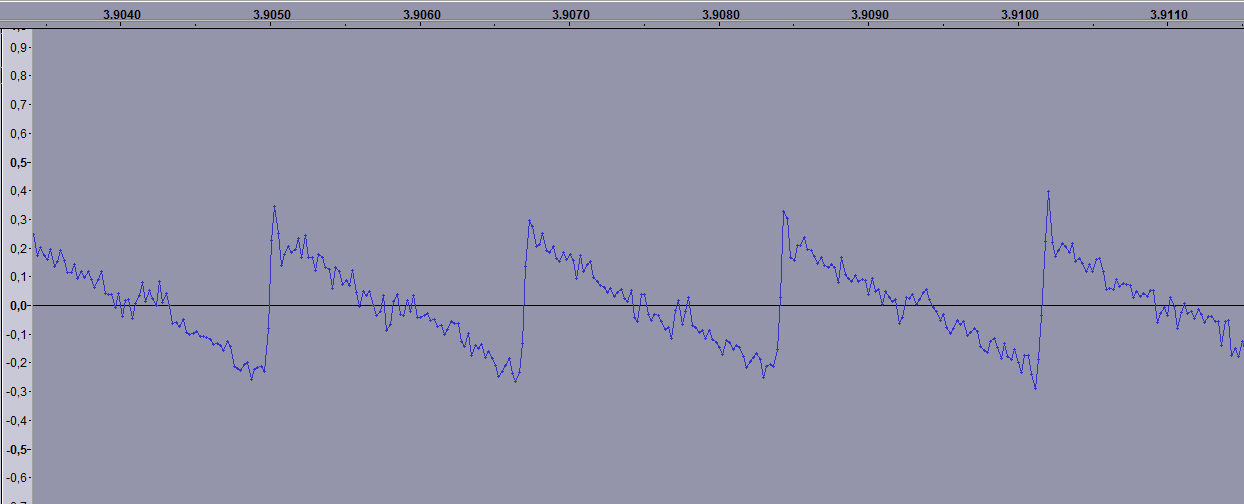
\includegraphics[width = \textwidth]{images/SW5zoom.png}
	\caption{A sawtooth wave}
	\label{img-sw5zoom}
\end{figure}

An ideal square wave is either at a maximum or minimum amplitude as seen in \ref{img-sw4zoom}, and shifts between them instantly.
Unlike a sawtooth wave, the square wave only contains odd-numbered integer harmonics.
\begin{figure}[H]
	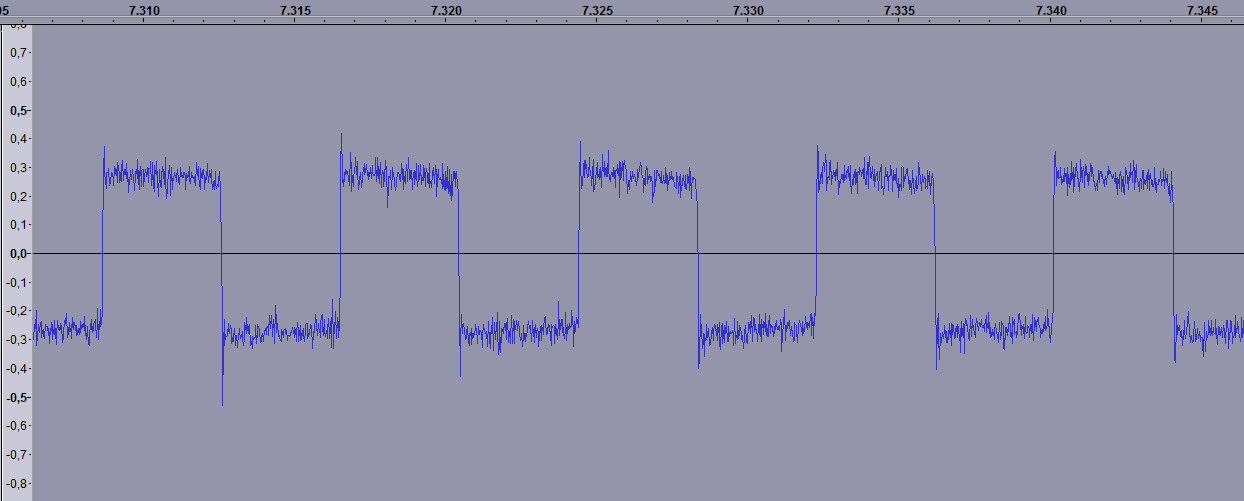
\includegraphics[width = \textwidth]{images/SW4zoom.png}
	\caption{A square wave}
	\label{img-sw4zoom}
\end{figure}

A noise is rather the lack of a waveform, with randomly chosen samples, as depicted in \ref{img-sw6zoom}.
Noise can be described as the sound your tv makes when you tune into frequencies that there is no broadcasting on.
\begin{figure}[H]
	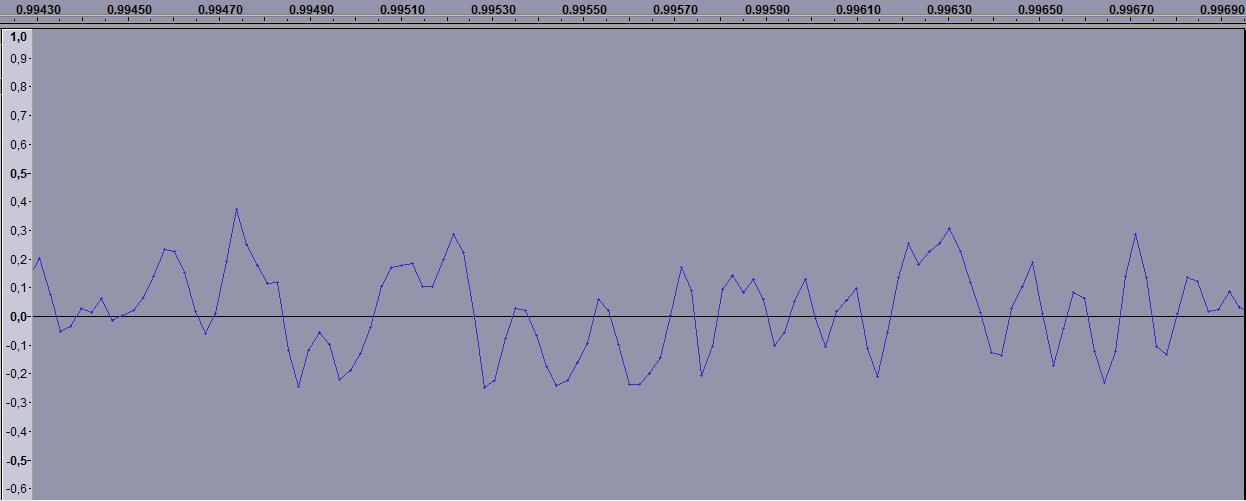
\includegraphics[width = \textwidth]{images/SW6zoom.png}
	\caption{A noise signal}
	\label{img-sw6zoom}
\end{figure}

In order to make sound effects we need more than just pure waves, as sound almost never consists of just a wave with constant amplitude.
It is the job of the ADSR envelope to solve this issue.
An envelope sets bounds for the amplitude of a wave, and an ADSR envelope divides the wave into four parts: attack, decay, sustain and release.

During the attack, the amplitude is gradually increased from 0 to a maximum value.
After the attack, the amplitude gradually decays to a sustain level, which is typically a fraction of the maximum value.
The sound stays at the sustain level for a given time, until it is released, and the amplitude gradually decreases until it reaches 0 again.

\subsubsection{Explosion}

`Explosion' is a NOISE-based sound effect with the following ADSR envelope:
\begin{itemize}
	\item{Attack: 0 ms}
	\item{Decay: 1000 ms}
	\item{Sustain: 0\%}
	\item{Release: 0 ms}
\end{itemize}
The effect is held for 0 ms.
The total length of the effect is $0 ms + 1000 ms + 0 ms + 0 ms = 1000 ms$.
`Explosion' can be triggered by pressing \texttt{SW6}.
The sound effect is depicted in \ref{img-sw6}.

\begin{figure}[H]
	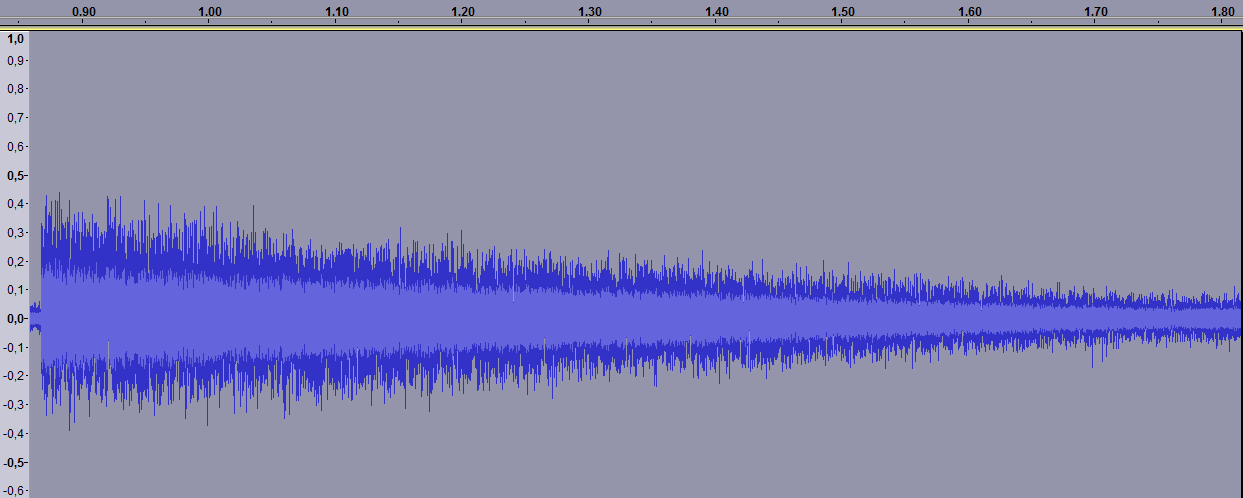
\includegraphics[width = \textwidth]{images/SW6.png}
	\caption{}
	\label{img-sw6}
\end{figure}


\subsubsection{Air horn}
`Air horn' is a SAWTOOTH-based sound effect with the following ADSR envelope:
\begin{itemize}
	\item{Attack: 100 ms}
	\item{Decay: 100 ms}
	\item{Sustain: 70\%}
	\item{Release: 500 ms}
\end{itemize}
The effect is held for 0 ms.
The total length of the effect is $100 ms + 100 ms + 500 ms + 0 ms = 700 ms$.
`Air horn' can be triggered by pressing \texttt{SW5}.
See \ref{img-sw5} for a visualization of `Air horn'.

\begin{figure}[H]
	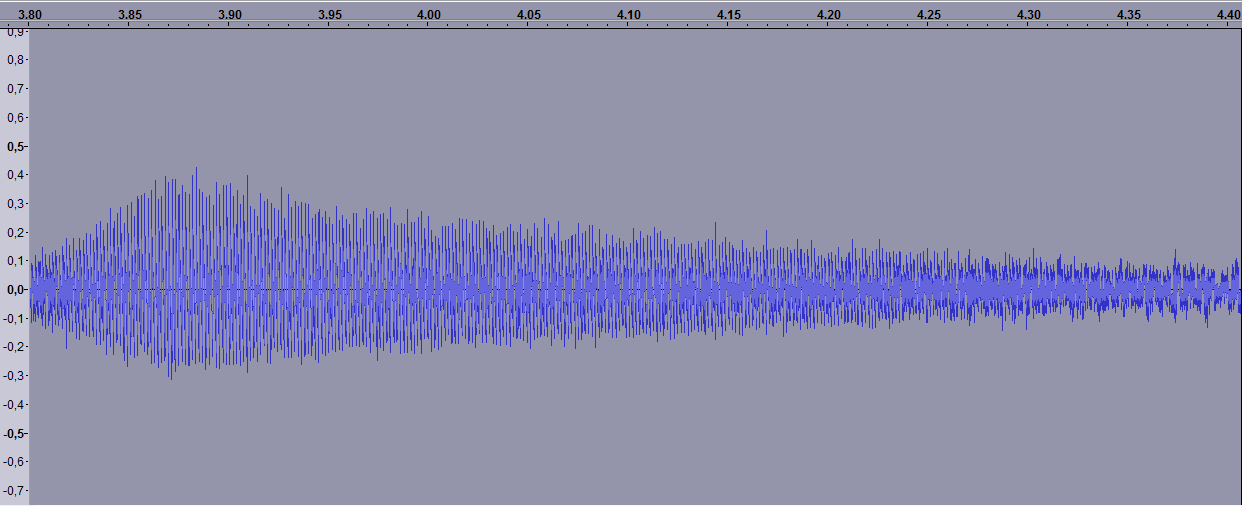
\includegraphics[width = \textwidth]{images/SW5.png}
	\caption{}
	\label{img-sw5}
\end{figure}

\subsubsection{Teleport}
`Teleport' is a SQUARE-based sound effect with the following ADSR envelope:
\begin{itemize}
	\item{Attack: 500 ms}
	\item{Decay: 1250 ms}
	\item{Sustain: 20\%}
	\item{Release: 250 ms}
\end{itemize}
The effect is held for 0 ms.
The total length of the effect is $500 ms + 1250 ms + 250 ms + 0 ms = 2000 ms$.
`Teleport' can be triggered by pressing \texttt{SW4}.
A picture of the recorded sound can be seen in \ref{img-sw4}.

\begin{figure}[H]
	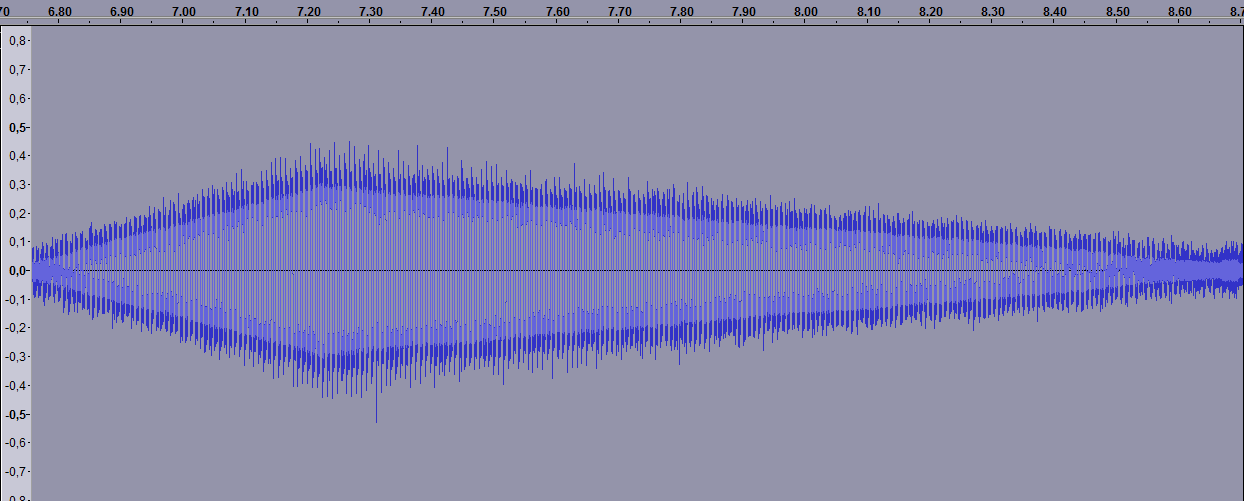
\includegraphics[width = \textwidth]{images/SW4.png}
	\caption{}
	\label{img-sw4}
\end{figure}


\subsection{Music}

The music pieces in the solution program are played by the MOD player.

\subsubsection{Tuulenvire by Dizzy/CNCD}
\emph{Tuulenvire} is a 2:09 long 808KB composition in the ambient genre, featuring piano and accordion, amongst other instruments.
This composition was chosen to demonstrate how careful composing can render realistic compositions with a relatively small memory footprint.
It uses 25 different PCM-coded sounds.
Tuulenvire can be triggered by pressing \texttt{SW3}.

\subsubsection{Boesendorfer P. S. S. by Romeo Knight}
\emph{Boesendorfer P. S. S.} is a 3:22 long 211KB solo piano composition, chosen to illustrate the possibilities enabled by a hybrid generative/recorded approach.
It uses 9 different PCM-coded sounds.
Boesendorfer P. S. S. can be triggered by pressing \texttt{SW2}.

\subsubsection{Drop The Panic by H0ffmann}
\emph{Drop The Panic} is a 4:05 long 702KB ``glitch-hop'' composition.
It was chosen to show how MOD files can support embedded vocals.
It uses 31 different PCM-coded sounds.
The composition was tweaked by adding some extra inaudible notes in the beginning of the song to decrease critical cache misses by the MOD player during playback on the STK1000.
Drop The Panic can be triggered by pressing \texttt{SW1}.

\subsubsection{Bacongrytor by Maktone}
\emph{Bacongrytor} is a 15Kb endless loop chiptune-style composition, chosen to demonstrate the compactness of the MOD format, and therefore its aptfulness for use on microcontrollers.
It uses 7 different PCM-coded sounds.
Bacongrytor can be triggered by pressing \texttt{SW0}.
